\documentclass[a4paper,12pt]{report}
\usepackage[latin1]{inputenc}   % Permet usar tots els accents i car�ters llatins de forma directa.
\usepackage[spanish]{babel}
%\decimalspanish{.}
\usepackage{latexsym}
\usepackage{hyperref}
\usepackage{theorem}
\usepackage{enumerate}
\usepackage{amsfonts, amscd, amsmath, amssymb}
\usepackage[pdftex]{graphicx}
\usepackage{epstopdf}
\usepackage{epsdice}

\setlength{\textheight}{23cm}
\addtolength{\topmargin}{-1.5cm}

\pagestyle{empty}
\begin{document}
\begin{center}
\textbf{\large Estad�stica Aplicada}

\textbf{\large Seguretat i Ci�ncies Policials}

\vskip 0.5 cm
\textbf{\large Activitat dirigida 2}
\end{center}

\vskip 1cm

%Consideram les  seg�ents dades sobre la classificaci� del RCD Mallorca durant la temporada 2006-07.
%
%\begin{center}
%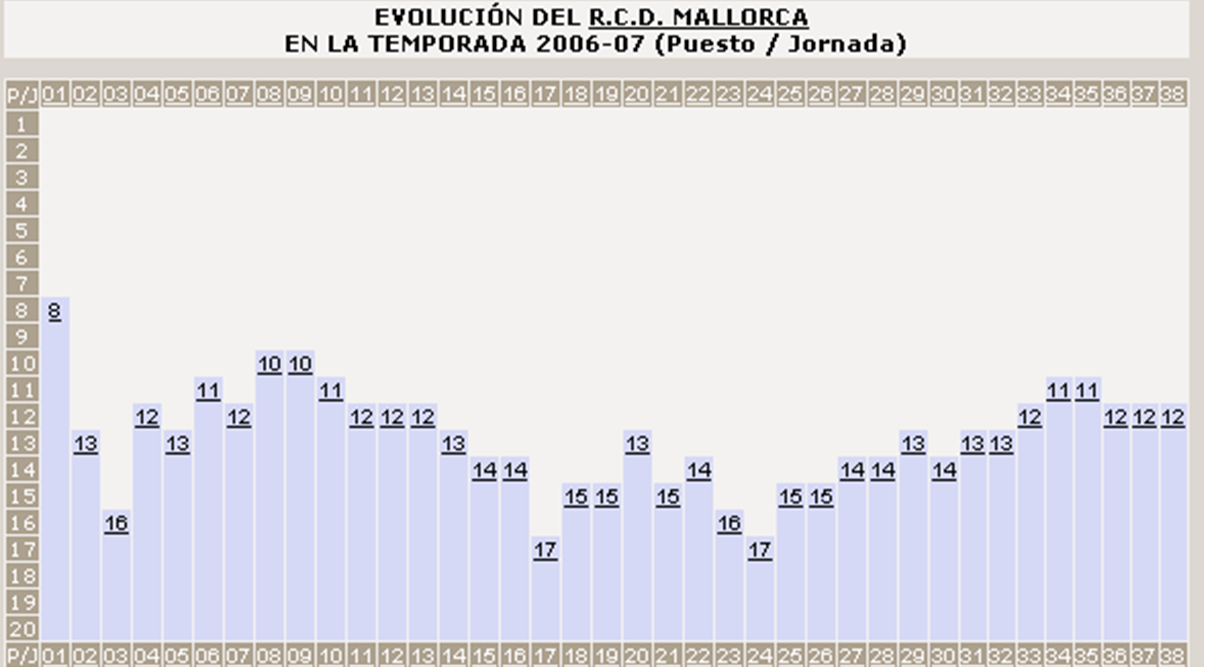
\includegraphics[width=12cm]{rcdmall0607.png}
%\end{center}
%
A partir dels resultats obtinguts en l'activitat 1 (taula de freq��ncies, quartils, mediana, mitjana, etc)
respon a les seg�ents q�estions:

\begin{enumerate}
\item Calcula el ratio de variaci�, el rang i el rang interquart�lic.

\item Dibuixa el diagrama de capsa, marcant els valors at�pics, si n'hi ha.

\item Calcula la vari�ncia i la desviaci� t�pica a partir de 
les dades brutes. Fes primer els c�lculs amb la calculadora i despr�s amb la fulla de c�lcul. 

\item Calcula la vari�ncia i la desviaci� t�pica a partir de
les dades de la taula de freq��ncies. Fes primer els c�lculs amb la calculadora i despr�s amb 
la fulla de c�lcul. 

\end{enumerate}


\end{document}